\documentclass[10pt]{exam}
\usepackage[hon]{template-for-exam}
\usepackage{tikz,multicol}

\title{Rotational Review Questions}
\author{Rohrbach}
\date{\today}

\begin{document}
\maketitle

\begin{questions}
\question
	If you are looking for each of the following, which symbol are you looking for and what conversions (if any) would you have to do?

  \begin{parts}
    \part
      Number of revolutions \vspace{2em}
    \part
      Rate of rotation in rpm \vspace{2em}
    \part
      Rate in rad/s$^2$. \vspace{2em}
    \part
      Linear velocity of a point on the outside of a wheel. \vspace{2em}
    \part
      Distance a wheel travels over a certain number of radians. \vspace{2em}
    \part
      Moment of inertia \vspace{2em}
    \part
      Angular momentum \vspace{2em}
    \part
      Torque \vspace{2em}
  \end{parts}


\question
	What would happen if a figure skater doing a pirouette were to pull in her arms?  Why? \vs

\question
	Use physics from this unit to describe why a nut is easier to loosen with a wrench than with your fingers. \vs

\question
	Why is the moment of inertia for a hoop larger than the moment of inertia for a disk? \vs

\pagebreak

\question
	Rank these object in terms of which would hit the bottom of a ramp first: a 5-cm diameter hoop, a 7-cm diameter hoop, a 5-cm diameter disk, a 7-cm diameter solid sphere.
  \vspace{10em}

\question
	Little Bobby and Janey are both riding a carousel.  Janey is on a pony, which is 5 m from the center of rotation, and Bobby is on a water buffalo, which is 7 m from the center. 

  \begin{multicols}{2}

    \begin{parts}
      \part
        Which child, if either of them, will have the greater $v$?  Explain. \vs
      \part
        Which child, if either of them, will have the greater $\omega$? Explain. \vs
    \end{parts}


    \begin{flushright}
      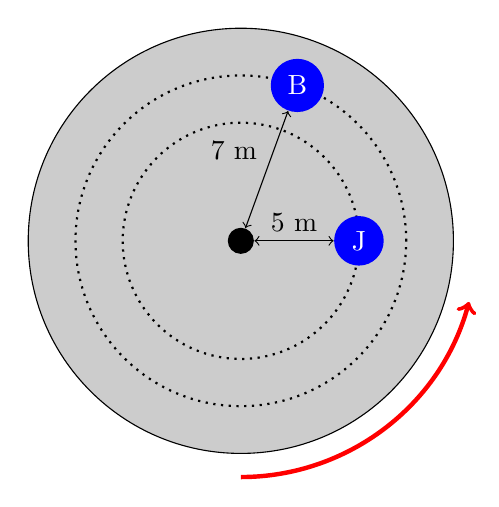
\begin{tikzpicture}[x=3mm,y=3mm]
        \draw[fill=gray!40] (0,0) circle (9);
        \node[circle,minimum size=0.5,fill=black] 
          at (0,0) (center) {};
        \draw[dotted,thick] (0,0) circle (5);
        \draw[dotted,thick] (0,0) circle (7);
        \node[circle,white,fill=blue] at (0:5)
          (Janey) {J};
        \node[circle,white,fill=blue] at (70:7)
          (Bobby) {B};
        \draw[<->] (center) -- (Janey) 
          node[midway,above] {5 m};
        \draw[<->] (center) -- (Bobby) 
          node[midway,above left] {7 m};

        \draw[->,ultra thick,red] (-90:10) arc (-90:-15:10);
      \end{tikzpicture}
    \end{flushright}

  \end{multicols}

\vspace{2em}


\question
	You are holding a spinning bicycle wheel while standing on a stationary, frictionless turntable.  The wheel is spinning counterclockwise with an angular momentum vector $\vec{L}_0$. 
  
  {\small (\emph{Image Credit: Giancolli} Physics with Applictations, \emph{7th e.})}

  \begin{minipage}[b]{.7\textwidth}
    \begin{parts}
      \part
        If you suddenly flip the wheel over, what will happen?  Why?
        \vspace{6em}
      \part
        What will the angular momentum of the turntable be in terms of $\vec{L}_0$? \vspace{4em}
    \end{parts}
  \end{minipage}
  %
  \hfill
  %
  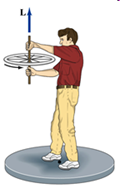
\includegraphics{bicycle-wheel.png}




  


\end{questions}

\end{document}